% Copyright 2004 by Till Tantau <tantau@users.sourceforge.net>.
%
% In principle, this file can be redistributed and/or modified under
% the terms of the GNU Public License, version 2.
%
% However, this file is supposed to be a template to be modified
% for your own needs. For this reason, if you use this file as a
% template and not specifically distribute it as part of a another
% package/program, I grant the extra permission to freely copy and
% modify this file as you see fit and even to delete this copyright
% notice. 

\documentclass[12pt]{beamer}
% Replace the \documentclass declaration above
% with the following two lines to typeset your 
% lecture notes as a handout:
%\documentclass{article}
%\usepackage{beamerarticle}
\usepackage[utf8]{inputenc}
\usepackage[noend]{algpseudocode}
\usepackage[T1]{fontenc}
\usepackage{algorithmicx}
\usepackage{amsmath}
\usepackage{mathtools}

% There are many different themes available for Beamer. A comprehensive
% list with examples is given here:
% http://deic.uab.es/~iblanes/beamer_gallery/index_by_theme.html
% You can uncomment the themes below if you would like to use a different
% one:
%\usetheme{AnnArbor}
%\usetheme{Antibes}
%\usetheme{Bergen}
%\usetheme{Berkeley}
%\usetheme{Berlin}
%\usetheme{Boadilla}
%\usetheme{boxes}
%\usetheme{CambridgeUS}
%\usetheme{Copenhagen}
%\usetheme{Darmstadt}
%\usetheme{default}
%\usetheme{Frankfurt}
%\usetheme{Goettingen}
%\usetheme{Hannover}
%\usetheme{Ilmenau}
%\usetheme{JuanLesPins}
%\usetheme{Luebeck}
%\usetheme{Madrid}
%\usetheme{Malmoe}
\usetheme{Marburg}
%\usetheme{Montpellier}
%\usetheme{PaloAlto}
%\usetheme{Pittsburgh}
%\usetheme{Rochester}
%\usetheme{Singapore}
%\usetheme{Szeged}
%\usetheme{Warsaw}

\title{Reconnaissance des chiffres}

\author{Nguyen Vaan Tho - Nguyen Quoc Khai}
% - Give the names in the same order as the appear in the paper.
% - Use the \inst{?} command only if the authors have different
%   affiliation.

% - Use the \inst command only if there are several affiliations.
% - Keep it simple, no one is interested in your street address.

\date{IFI, Hanoi, 2013}
% - Either use conference name or its abbreviation.
% - Not really informative to the audience, more for people (including
%   yourself) who are reading the slides online

\subject{Reconnaissance des chiffres}
% This is only inserted into the PDF information catalog. Can be left
% out. 

% If you have a file called "university-logo-filename.xxx", where xxx
% is a graphic format that can be processed by latex or pdflatex,
% resp., then you can add a logo as follows:

% \pgfdeclareimage[height=0.5cm]{university-logo}{university-logo-filename}
% \logo{\pgfuseimage{university-logo}}

% Delete this, if you do not want the table of contents to pop up at
% the beginning of each subsection:
\AtBeginSubsection[]
{
  \begin{frame}<beamer>{Plan de présentation}
    \tableofcontents[currentsection,currentsubsection]
  \end{frame}
}

% Let's get started
\begin{document}

\begin{frame}
  \titlepage
\end{frame}

\begin{frame}{Plan de présentation}
  \tableofcontents
  % You might wish to add the option [pausesections]
\end{frame}

\section{Introduction}
\begin{frame}{Introduction}
  \begin{itemize}
  \item Reconnaître des chiffres manuscrits
  \item Plein de recherches qui donnent les résultats efficaces : K-plus proches voisins, Classification non linéaire, SVM, Réseaux neuraux, etc.
  \item Nous cherchons des méthodes qui
  \begin{itemize}
   \item rendent des résultats acceptables
   \item sont faisable
  \end{itemize}
  \end{itemize}
  
\end{frame}


\begin{frame}{Introduction}
  \begin{itemize}
  \item Nous allons implémenter 2 algorithmes en C++ et OpenCV
  \begin{itemize}
   \item KNN 
   \item SVM 
  \end{itemize}
  \item Nous allons expérimenter plusieurs configurations des paramètres de chaque 
méthode pour trouver les meilleures paramètres 
  \end{itemize}
  
\end{frame}

\section{Rappel de KNN et SVM}
\subsection{KNN}
\begin{frame}{K-plus proches voisins}
Cette méthode est réalisé dans des étapes suivantes.
\begin{block}{Détection des blocks}
Diviser l'image en N blocks de même taille. Choix $N = 14x14 = 196$.
\end{block}

\begin{block}{Calcul du descripteur}
Un descripteur contient $N$ éléments. 
\begin{equation}
D = \sqrt{\sum_{\substack{
   	(1<=i<=N)}} (e_{1i} - e_{2i})^2}
\end{equation}
\end{block}

\begin{block}{K-plus proches voisins}
Prendre $K$ images ayant les distances les plus courtes. Choix du type le plus populaire pour le type de l'image de test.
\end{block}
\end{frame}


\subsection{SVM}
\begin{frame}{SVM}
\begin{center}
 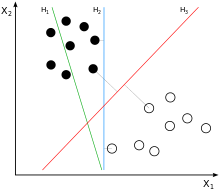
\includegraphics[width=4cm]{./images/svmc.png}
\end{center}

\begin{center}
 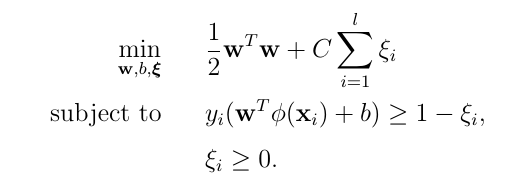
\includegraphics[width=6cm]{./images/svm.png}
\end{center}

Le kernel gaussien utilisé dans notre programme:
\begin{center}
$K(x_{i}, x_{j}) = exp(-\gamma(x_{i}- x_{j})^2)$
\end{center}
\end{frame}

\section{Expérimentation}
\subsection{Critères d'évaluation}
\begin{frame}{Critères d'évaluation}
  \begin{itemize}
  \item Pour évaluation notre programme, nous utilisons 2 critères
  \begin{itemize}
   \item Le taux de précision
   \item Le temps de calcul 
  \end{itemize}
  \end{itemize}
\end{frame}
\begin{frame}{Données}
  \begin{itemize}
	\item Base d'apprentissage 5000 images
	\item Base de test 1000 images
  \end{itemize}
\end{frame}

\subsection{Méthode KNN}
\begin{frame}{Méthode K-NN}
Bien choisir des paramètres comme le nombre de block, le K plus proches voisins.
\begin{block}{Nombre de block}
Quand le nombre de block est petit ou très grand, le résultat n'est pas exact. $N = 14x14$
\end{block}
\begin{block}{K}
K plus proches voisins, le bon est de 4.
\end{block}
\end{frame}

\subsection{Méthode SVM}
\begin{frame}{Les paramètres}
  \begin{itemize}
   \item C
   \item gamma
   \item nombre de blocs
  \end{itemize}
\end{frame}

\begin{frame}{Les paramètres}
  Pour trouver les meilleures paramètres nous avons expérimenté plusieurs valeurs de ces 
paramètres en deux boucles:

Première boucle:
  \begin{itemize}
   \item C = $2^{-5}$ à $2^{15}$
   \item gamma = $2^{-19}$ à $2^3$
   \item nombre de blocs = 7
  \end{itemize}
Deuxième boucle, utilisation de résultat de première boucle:
  \begin{itemize}
   \item C = 2 à 8
   \item gamma = 0.0004 à 0.04
   \item nombre de blocs = 7 à 14
  \end{itemize}

\end{frame}

\section{Résultats}
\subsection{Méthode KNN}
\begin{frame}{Méthode K-NN}
\begin{figure}[!htb]
\minipage{0.55\textwidth}
  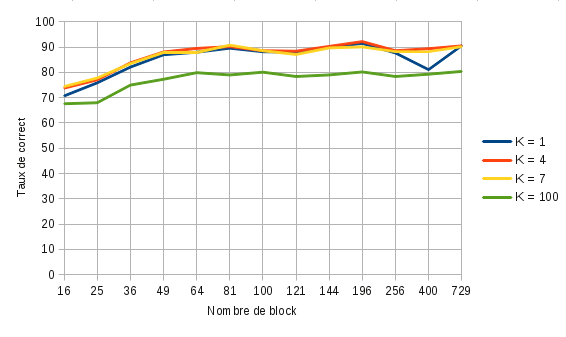
\includegraphics[width=\linewidth]{images/graphique.png}
  \caption{Taux de prédition}\label{fig:awesome_image2}
\endminipage\hfill
\minipage{0.55\textwidth}
  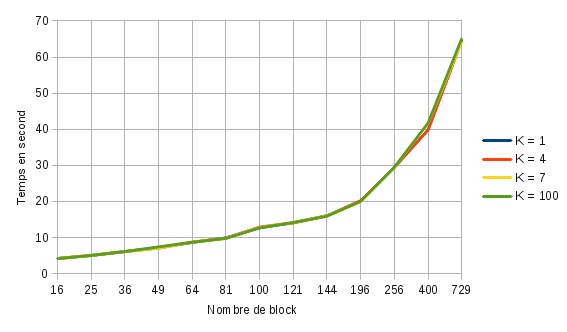
\includegraphics[width=\linewidth]{images/graphique1.png}
  \caption{Temps de calcul}\label{fig:awesome_image3}
\endminipage\hfill
\end{figure}
\end{frame}

\subsection{Méthode SVM}

\begin{frame}{Résultats SVM}
 \begin{figure}[ht]
	\begin{center}$
		\begin{array}[h]{cc}
		  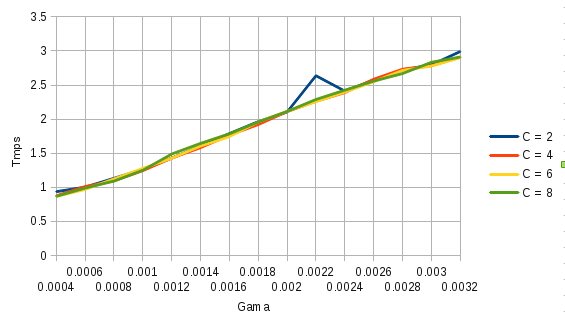
\includegraphics[width=4.5cm]{images/graphique2.png}&
		  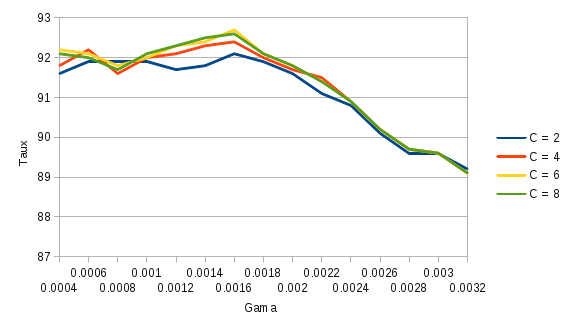
\includegraphics[width=4.5cm]{images/graphique3.png}
		\end{array}$
	\end{center}
	\caption{Taux de précision, temps de calcul avec blocs = 7x7}
 \end{figure}

 \begin{figure}[ht]
	\begin{center}$
		\begin{array}[h]{cc}
		  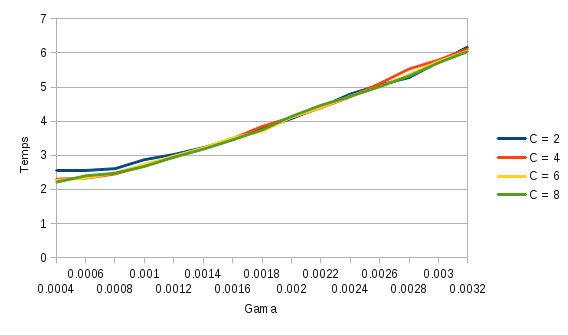
\includegraphics[width=4.5cm]{images/graphique4.png}&
		  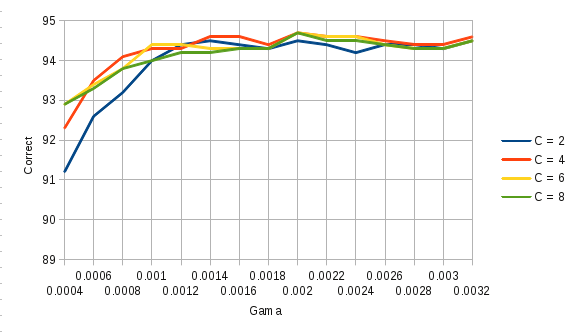
\includegraphics[width=4.5cm]{images/graphique5.png}
		\end{array}$
	\end{center}
	\caption{Taux de précision,temps de calcul avec blocs=14x14}
 \end{figure}

\end{frame}
\subsection{Comparaison entre KNN et SVM}
\begin{frame}{Comparaison entre KNN et SVM}
\begin{itemize}
 \item SVM est beaucoup plus vite 
 \item SVM est un peu plus précisément 
\end{itemize}

\end{frame}
\section{Conclusion}
\begin{frame}{Conclusion}
\begin{itemize}
\item Dans ce projet, nous avons implémenté deux méthodes basant sur l'algorithme KNN et 
SVM
\item Nous avons expérimenté plusieurs configurations des paramètres et comparer les deux 
méthodes
\end{itemize}
\end{frame}

% All of the following is optional and typically not needed. 
\section*{Références}

\begin{frame}
\begin{thebibliography}{9}
\bibitem{c1}
  David Lowe
  \emph{THE MNIST DATABASE of handwritten digits}.
  Yann LeCun, Courant Institute, NYU,
  Corinna Cortes, Google Labs, New York,
  Christopher J.C. Burges, Microsoft Research, Redmond,
  \emph{http://www.cs.ubc.ca/~lowe/keypoints/}
   
\bibitem{c2}
  Chih-Wei Hsu, Chih-Chung Chang, and Chih-Jen Lin
  \emph{A Practical Guide to Support Vector Classification}.
  Department of Computer Science
National Taiwan University, Taipei 106, Taiwan
  \emph{http://www.csie.ntu.edu.tw/~cjlin}
 
\end{thebibliography}
\end{frame}
\begin{frame}
 \Huge Merci pour votre attention!
\end{frame}

\end{document}
